\documentclass[../main/main.tex]{subfiles}

\newdate{date}{11}{12}{2020}


\begin{document}

\marginpar{ \textbf{Lecture 22.} \\  \displaydate{date}. \\ Compiled:  \today.}

\subsection{$\pmb{R_0}$ from the cluster size}

We will now provide another tool to estimate $R_0$: we will try to infer it from the \textbf{cluster size}. This is useful specially when \textit{infections are not highly transmissible}, that is to say when we do \textbf{not} observe an \textbf{exponential growth} of cases, but only sporadic infections.

Let us discuss which are the possible infections with $R_0<1$, in particular what are their main features. These are for example \textit{zoonotic infections}, such as $MERS$\footnote{Middle East Respiratory Sindrome (MERS) coronavirus, 2013. Breban, et al. The Lancet 2013 } that was transmitted through dromedaries and camels and whose mortality rate was high, or infections that are \textit{close} to \textit{eradication threshold}, such as measles. It is important to analyze such diseases and to understand how far we are from the epidemic threshold, since the higher the number of infected individuals, the higher the risk of a mutation in the pathogen or a decrease in vaccine uptake.

We want to understand how to deal with this problem: a first approach is to \textit{assume} that the \textit{few cases} we observe are \textbf{linked} to a \textbf{unique cluster}.

We define as a \textbf{cluster} all cases generated by the so called \textit{index case}. A cluster is an entity like the one in Fig. \ref{fig:22_01}, whose most important quantities are:
\begin{itemize}
    \item \textbf{Index case}: infection caused by an external source.
    \item \textbf{Offsprings}: cases infected by the index case.
\end{itemize}
In the case where we deal with many clusters, the distribution of their size $s$ depends on $R_0$ according to $P(s|R_0)$.

\begin{figure}[h!]
\centering
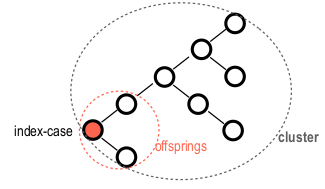
\includegraphics[width=0.50\textwidth]{../lessons/image/22/image01.png}
\caption{\label{fig:22_01} Estimation of $R_0$ using a cluster approach when observing a small amount of cases.}
\end{figure}

Some examples of $P(s|R_0)$ probability density might be, depending on the assumptions we make on the heterogeneity of the network:
\begin{itemize}
    \item All infectious individuals behave equally and generate on average $R_0$ transmissions. The number of \textit{offsprings} is $k$ and are distributed as a Poisson:
    \begin{equation*}
        k \sim \text{Pois}(k|R_0) \implies P(s|R_0) = \frac{(sR_0)^{s-1}e^{-sR_0}}{s!}
    \end{equation*}
    \item Introducing a \textit{continuous-time} $SIR$ dynamics, since $R_0$ is below 1 stochastic effects are important. The size of the cluster therefore follows a \textit{Markovian birth and death process} of the kind:
    \begin{equation*}
        P(s|R_0) = \frac{(2s - 2)!}{s!(s-1)!} \frac{R_0^{s-1}}{(R_0 + 1)^{2s-1}}
    \end{equation*}
\end{itemize}
However, it might happen, specially when cases are few, that many of them are not reported: data we have is almost for sure biased in this sense. Hence we need to account also for \textbf{under-reporting}. Each case may go unobserved with probability $p_{miss}$: as a consequence if a cluster has real size $s$, we may observe a cluster of size $o \leqslant s$.

The \textbf{probability of observing a cluster} of size $o \geqslant 1$, given $R_0$, is Binomial wrt missed cases:
\begin{equation*}
    P(o|R_0, p_{miss}, o\geqslant1) = \frac{\sum_{s\geqslant 0} P(s|R_0) \binom{s}{o}p_{miss}^{s-o}(1-p_{miss}^o)}{1-o(o=0|R_0, p_{miss})}
\end{equation*}
where $P(s|R_0)$, can be any of the aforementioned probabilities. And the \textbf{likelihood}:
\begin{equation*}
    \mathcal{L}(o_i|R_0, p_{miss}) = \left( \sum_i o_i \right)! \prod_i \frac{1}{o_i !} P(o|R_0, p_{miss}, o\geqslant 1)
\end{equation*}
where, as an example, the first factor sums over all the possible sizes of the cluster that we may have observed, and all the possible permutations ($"!"$).

Exploiting the tools we have just introduced epidemiologists were able to provide an estimate for $R_0$. It is interest to notice that at early spread, in February this was $R_0 \simeq 2$. More likely the $R_0$ for the Eastern strain of Coronavirus was computed. Indeed a couple of months later scientists were able to estimate $R_0$ for the European strain, and it resulted to be $R_0 \simeq 3$. This can explain why in UK the Chinese strain was overtaken by the European one, despite it appeared earlier and number of infected people was way larger.


\section{Incubation period estimation}

One other relevant quantity we need to estimate as soon as possible is the \textbf{incubation period}. It is really important since, under some assumptions, we can relate it to the \textit{generation times} distribution from which to compute $R_0$. In order to do it, high quality data is needed. However, if there is none, we can still provide an estimation by using similar diseases one, even though obviously this analysis might lead to wrong outcomes.

\begin{figure}[h!]
\centering
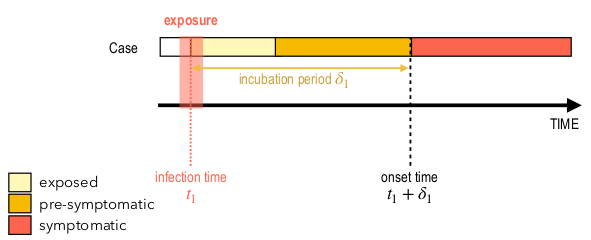
\includegraphics[width=0.90\textwidth]{../lessons/image/22/image02.png}
\caption{\label{fig:22_02} Incubation period analysis.}
\end{figure}

The \textbf{incubation time} is defined as the time elapsed between the \textbf{onset} of symptoms and the \textit{infection time}, namely when the \textbf{exposure} occurred (Fig. \ref{fig:22_02}).
The former is easy to collect, for instance when a person has been visited by a doctor and start showing any symptoms. In addition, incubation time is also a measure of the delay in the response of restriction policies in infection curve. However, exposure time is very difficult to retrieve, nonetheless is very important: pre-symptomatic phase relevance is even higher for COVID-19, since pre-symptomatic individuals turn out to be really infectious.  Some ways deal with this problem are through \textbf{contact tracing}, \textbf{case investigation}. Once a case is confirmed, contacts are investigated. They are contacted, isolated and go through clinical and virological assessment. This allows us to collect infector-infected pairs and more likely when contact occurred.

One other approach one may want to follow to estimate the \textit{incubation period} is to proceed with the \textbf{analysis of travelling cases}. With referral to Fig. \ref{fig:22_03} and COVID-19 outbreak: Backer et al.\footnote{Backer, Klinkenberg, Wallinga. Incubation period of 2019 novel coronavirus (2019-nCoV) infections among travellers from Wuhan, China, Euro Surveill. 2020;25(5).} analyzed 88 cases detection starting from January, 20th through January, 28th. Their travel history (to and) from Wuhan was known, as well as their symptom onset date. During this early stage of the epidemic, it is most likely that travellers were infected in Wuhan. Consequently, their time spent in Wuhan can be assumed to be the duration of exposure to infection without any contact tracing procedure.
As said, we know \textit{for sure} the date of the onset of symptoms, but we need to infer when infection occurred. One should note that the shorter the stay in a risky area, the more precision we have in inferring the duration of infection period. After providing these estimations, data was fitted and compared using 2-parameter continuous distributions supported on a semi-infinite intervals, such as Gamma, Weibull and Log-normal distribution. Later, they proceeded to maximize the Likelihood and, by the means of a strictly positive flat prior for the two parameters, since there was no guess about their value, they tried to infer them. The most credible estimation for the \textbf{incubation period} was:
\begin{equation}
    \text{incubation period} \ \sim 6.4 \text{ days} \qquad \text{C.I. 95\%}[2.1, 11.1]\text{ days}
\end{equation}

\begin{figure}[h!]
\centering
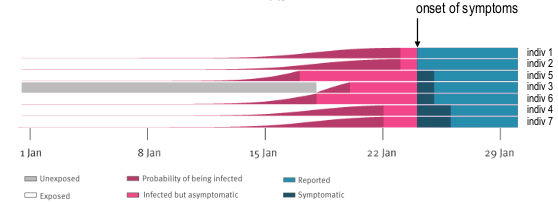
\includegraphics[width=0.90\textwidth]{../lessons/image/22/image03.png}
\caption{\label{fig:22_03} Pioneer analysis of travelling cases for COVID-19 outbreak.}
\end{figure}




\section{Generation time and serial interval estimation}

Let us recall the definition of the \textbf{generation time}: it is the time elapsed between the moment when the infector was infected and the moment when he infects someone as one can see in Fig. \ref{fig:22_05}).
It is indeed really difficult to obtain, nonetheless it can be computed thanks to the \textbf{serial interval} $T_s$ that are easier to compute. It is the time \textit{elapsed} between the \textit{onset of symptoms} for two individuals, where we assume one to be the infector and the other one the infected. Therefore, the serial interval is a random variable that is linked to both generation times distribution ($\tau$) and the incubation periods distribution ($\delta$) in the following way:
\begin{equation}
    \tau_S = \overset{\text{onset time case 2}}{(t_2 + \delta_2)} - \overset{\text{onset time case 1}}{(t_1 + \delta_1)} = \underset{\text{serial interval}}{(t_2 - t_1)} + (\delta_2 - \delta_1) = \tau + (\delta_2 - \delta_1)
\end{equation}
where we sample $\tau \sim w(\tau|\theta_2)$, $\delta \sim g(\delta|\theta_1)$, $\tau_s \sim f(\tau_s|\theta_1,\theta_2)$.
This indeed is true \textit{on average}, and can be done since we assume that the average generation time and the average infectious duration are equal. Therefore, \textbf{serial interval} is often used as a \textbf{proxy} for the \textbf{generation time}, but with a warning! This argument is valid since $\expval{\delta_1} = \expval{\delta_2}$, therefore $\expval{(\delta_2 - \delta_1)} = 0$, but we should recall that $\tau_S \neq \tau$: \textit{on average} they are the same ($\expval{\tau_s} = \expval{\tau}$), but their \textit{variance} is different ($\sigma_{\tau_S}>\sigma_\tau$)
\footnote{Indeed, $Var(X+Y) = Var(X)+Var(Y)$.}!

\begin{figure}[h!]
\centering
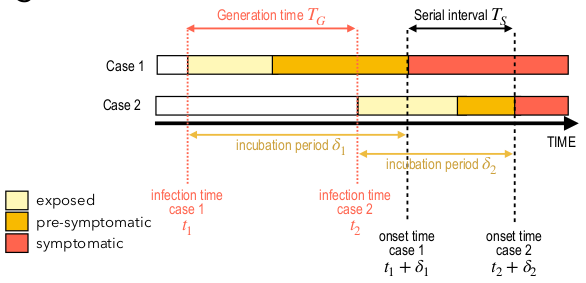
\includegraphics[width=0.90\textwidth]{../lessons/image/22/image05.png}
\caption{\label{fig:22_05} Generation time and serial interval relation. }
\end{figure}

Moreover, the variance of the generation times distribution $f$ is greater than the one of $w$ of infectious duration: indeed we can observe infections even caused by pre-symptomatic individuals: \textbf{pre-symptomatic phase} is important for transmission. In addition, variance of $f$ is also greater than the variance of $G$ and this might lead to an underestimation of $R_0$ since it holds that, relating the latter to the serial interval distribution, $R_0 \simeq e^{GT_G - (1/2)G^2 \sigma^2}$.

As an example, let us consider the case of COVID-19 data and proceed with the estimation of the generation times distributions. Researchers\footnote{Ganyani, Kremer, Chen, Torneri, Faes, Wallinga, Hens. Estimating the generation interval for coronavirus disease (COVID-19) based on symptom onset data, Euro Surveill. 2020;25(17):pii=2000257} reported $91$ confirmed cases in Singapore and $135$ in Tianjin, and relied their paper on previous estimates of incubation period, whose distribution is:
\begin{equation}
    \delta \sim g(\delta|\theta_1) = \text{Gamma}(\delta|\theta_1)
\end{equation}
Data we are talking about consisted in information about infector and infected pairs. We know that \textbf{generation times} is $\tau_S = \tau + (\delta_2 - \delta_1)$, therefore distributes according to the convolution between the two distributions $h$ and $w$:
\begin{equation}
    f(\tau_S|\theta_1, \theta_2) = \int_{-\infty}^{+\infty} w(\tau - x|\theta_2) h(x|\theta_1) dx = \mathcal{L}(\{\tau_{s,i}\}|, \theta_2 \theta_1)
\end{equation}
where $x = \delta_2 - \delta_1$, $x\sim h(x|\theta_1)$ and $\{\tau_{s,i}\}$ is the set of generation intervals observed.

Once we have proceeded to the estimation of $\theta_2$ we can numerically compute:
\begin{equation}
    P(t_2 < t_1 + \delta_1) = P(\tau_S < \delta_1)
\end{equation}
that gives us the \textbf{proportion of cases generated by pre-symptomatic transmission}. The final results are the following for the COVID-19:
\begin{equation}
    \text{generation time } = 5.20 \text{ days} \qquad \text{C.I. 95\% }[3.78-6.78] \text{ days}
\end{equation}
and the \textit{proportion of pre-symptomatic transmission} being around $50\%$, that is a high number. This implies that infected people tend to infect more if they are not reported, since this number is not negligible. A natural consequence is that, when we spot a case, it will have already infected almost half of the people it would infect during the whole infectious period.

The opposite case actually tells us why Ebola did not spread: despite a really high mortality rate ($60-70\%$), the infectiousness was not constant in time and was proportional to the time individuals stay infected as long as with the severity of the symptoms. Those individuals could be successfully isolated in time as soon as any symptom shows up, thus avoiding the spread. In this case, \textbf{isolation} for infected individuals is a successful solution to stop the disease.



\section{Infection severity}

One of the most important quantities we may want to compute is the \textbf{infection severity}. Indeed, we need to know the full spectrum of symptoms including the ones of \textbf{pauci-symptomatics} and \textbf{asyntomatics}. It gives us a key to interpret data and observations, moreover allows us to estimate the \textbf{actual number of infections} and its \textbf{cumulated}: this might be helpful to understand how many people are susceptible to the disease at the moment. Another reason to explain why it is important is if, once recovered, we acquire some sort of immunity, even temporary, actual susceptible people become less in number. Moreover, it is important to compute the \textbf{infection fatality ratio} and to provide \textbf{projections on hospital needs}: we will know how many people would need ICU or hospitalization, based on the fraction of people that develop mild or more serious illness. These fractions are normalized wrt \textit{total} number of infected people, including asymptomatic, so one should easily understand how much hard is to compute these ratios.

On the other hand this is a really difficult task to estimate these proportions, but this goal can be pursued through \textbf{contact tracing studies}, routine testing, or cohorts\footnote{We choose a sample of people/volunteers among a population, and proceed to follow their evolution in time in terms of infected, recovered, times distributions and so on.}. Indeed these are actually very difficult and expensive procedures, specially in terms of resources, and may require even formation for people which were assigned by these task. Moreover some natural experiments could be done. That is the case of the \textit{Diamond princess}, a cruise ship in Japan where some people were tested positive. Therefore, others were quarantined on the boat for some time: eventual infections were registered, reported their eventual symptoms and finally led to the hospital. However, this brought someone to raise some ethical objections over this scientific non conventional approach. Another experiment was due to repatration flights, where people were tested in airports while returning home in addition to the reporting of their eventual symptoms.

In conclusion, the \textit{true proportion} of asymptomatics of COVID-19 is still not certain $(\sim 20\%-50\%)$ and there is a strong dependence on age.



\section{Reproductive ratio $\pmb{R_t}$}

Let us compute the most relevant quantity of the epidemiological process, namely the \textbf{Reproductive ratio} $R_t$. This is different from the \textbf{basic reproductive ratio} $R_0$ and we recall that the latter is average number of cases an infectious individual infects in a \textit{fully susceptible population} during the course of his/her infectious period. Moreover, this is \textit{computed at the initial stage of an outbreak}. However, this is not realistic, being the number of susceptible dependent on time, for instance due to acquired immunity.

Instead, the \textbf{Reproductive ratio} $R_t$ is the \textbf{average number of cases} an infectious individual infects \textbf{at a given time} $t$ during the course of his/her infectious period. This is the \textit{natural extension} of $R_0$ to the later outbreak stage. It is an \textbf{indicator} of how the transmission potential of the epidemic evolves in time.

The \textbf{dependence in time} has to be introduced to take into account that as the outbreak unfolds the population is not fully susceptible anymore. We retrieve the simple version of the Kermack and McKendrick model, where the new infections:
\begin{equation}
    I(t+\delta t) = I(t) e^{\left[ \mu \int_t^{t+\delta t} \left( R_0 \frac{S(t')}{N(t')} - 1 \right) dt' \right]}
\end{equation}
That in turn can be locally approximated to:
\begin{equation}
    I(t+\delta t) \simeq I(t) e^{\delta t \mu (R_t - 1)}
\end{equation}
where $R_t = R_0 \frac{S(t)}{N(t)}$.

In reality things are more complex: $R_t$ does not change only due to the depletion of susceptible (immunity building): it might change as effect of interventions, behavioural change of population ($\expval{k_t}$ term):
\begin{equation}
    R_0 = \frac{\beta \expval{k}}{\mu} \longrightarrow R_t = \frac{\beta \expval{k_t}}{\mu} \frac{S(t)}{N(t)}
\end{equation}

Now, we drop the assumption of the simple $SIR$ and put ourselves in a more general framework. We will follow two different paths and interpretations to compute $R_t$.


\subsubsection{Cori method}

The first one is the method used almost in all Western countries, and was developed by \textbf{Cori} et al.\footnote{Cori, Ferguson, Fraser, Cauchemez, A New Framework and Software to Estimate Time-Varying Reproduction Numbers During Epidemics, American Journal of Epidemiology, 178, 2013.}.
The main pro is that it captures immediate changes in number of contacts thanks to lockdown or other restrictions, and this makes it really useful. It starts from a generic generation time distribution, namely $w(\tau)$, and it is based on the Lotka Euler equation:
\begin{equation}
    I(t) = \int_0^\infty I(t-\tau) \beta(\tau) d \tau
\end{equation}
where $\beta(\tau) = w(\tau)R_0$. One should note that the number of infected people at time $t$ depends on the number of infected at time $t-\tau$ and on the model parameters at time $\tau$!

Let us generalize the last expression. In order to do so, we make the assumption that the reproductive ratio varies in time, being the infectiousness time dependent as well $\beta (\tau,t) = w(\tau)R_t$. Therefore introducing $R_t$:
\begin{equation}
    I(t) = \int_0^\infty I(t-\tau) w(\tau) R_t d\tau
\end{equation}
note as it was introduced the dependence over the absolute time $t$ through the variable $R_t$.

Reverting the last equation and discretizing the time we obtain:
\begin{equation}
    R_t = \frac{I_t}{\sum_{s=1}^t I_{t-s}w_s}
\end{equation}
where the denominator indicates the total infectiousness of individuals that are infectious at the time $t$.
According to this \textbf{interpretation}, $R_t$ \emph{is the average number of secondary cases that each infected individual would infect if the} \textbf{conditions remained as they were at time t}.
This method is called “\textbf{real time method}”, since it links the actual situation to the past one through the generation times distribution finally providing an estimation for $R_t$. Given the total number of newly infected people today we can assume that background situation will not change in the close future, finally trying to predict the future number of infections that is function of $R_t$.
The \( R_t \) analysis in France is illustrated in Fig. \ref{fig:22_06}.

\begin{figure}[h!]
\centering
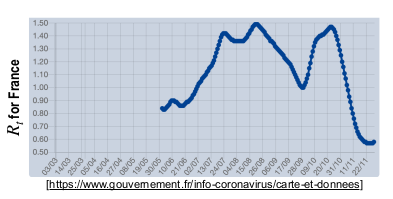
\includegraphics[width=0.60\textwidth]{../lessons/image/22/image06.png}
\caption{\label{fig:22_06} $R_t$ analysis for France throughout 2020. Changes are mainly due to restriction and variation of $\expval{k_t}$ and most likely not due to immunity building.}
\end{figure}


\subsubsection{Wallinga method}

The second interpretation we introduce is the one made by \textbf{Wallinga} et al.\footnote{Wallinga, Teunis, Different Epidemic Curves for Severe Acute Respiratory Syndrome Reveal Similar Impacts of Control Measures, American Journal of Epidemiology, 160, 6, 2004.}. It is used to infer \textit{who infected whom} from available information. When we have an incidence curve, the \textbf{only information} regarding a case is the \textbf{date} in which a case was recorded. Hence, the relative \textbf{probability} $p_{ij}$ that case $i$ is infected by case $j$, given the time elapsed $t_i - t_j$ depends on the \textbf{generation interval} and assuming a case is registered the date in which it was infected is:
\begin{equation}
    p_{ij} = \frac{w(t_i - t_j)}{\sum_{i \neq k} w(t_i - t_k) }
\end{equation}
The denominator denotes all the case we have, and acts as a sort of normalization term. Sometimes, however, this is not realistic since there might be some delays in reporting the cases. We now introduce the \textbf{cohort reproduction number}:
\begin{equation}
    R_j = \sum_i p_{ij}
\end{equation}
it counts the \textit{average number of secondary transmissions caused by a cohort} that was infected at time step $t$. It is the infection potential of a cohort (might be even a single individual) at time $t$. We recall that a cohort is \textit{not} a cluster, but is a group of cases that we follow from now on in the future, as a sample individuals. This method takes into account naturally the variability in the transmission potential of all individuals, since we are not making any assumption for it. We are trying to quantify \textbf{number of transmission generated by cases at time }$t$.

The \textbf{price to pay} for using this method is that it can be used \textbf{only retrospectively}: we are trying to compute when the secondary cases, generated by the infected at time $t$, have already been infected.

\subsubsection{Method comparison}

\begin{figure}[h!]
\centering
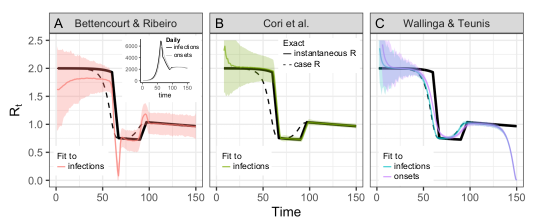
\includegraphics[width=0.90\textwidth]{../lessons/image/22/image07.png}
\caption{\label{fig:22_07} Difference between Bettencourt, Wallinga and Cori approaches for computing $R_t$. We see that Wallinga's has a cut-off. This behavior was expected since this approach analyzes future cases that are manually set to 0, nonetheless this kind of estimation is wrong. Cori's instead is more realistic.}
\end{figure}

We now want to make a little comparison between the two above described models (Fig. \ref{fig:22_07}).

 % (see fig. \ref{fig:22_08} for some output images\footnote{Practical considerations for measuring the effective reproductive number, $R_t$, Gostic, McGough, Baskerville, Abbott, Joshi, et al medRxiv 2020.}).

\textbf{Cori} describes the number of new infections at time $t$ and link them to \textit{past infections}. Hence, it \textbf{look backwards in time}. On the other hand, \textbf{Wallinga} relates the number of today's infections at time $t$ to the \textit{future cases} they will generate. Hence, it \textbf{looks forward in time}. The last model however cannot be used in real time analysis, but it sticks more to the $R_t$ definition.


Let us use these approaches with a more practical task. Let us compute the actual life span of some individuals that was born in 2013. Using Wallinga's retrospective approach, we would need to wait until all individuals die out, and then proceed to estimation. Conversely, using Cori's approach, we could estimate the same quantity by assuming that death rates in the future will be similar to present ones. It is a more physical approach: indeed it takes into account actual conditions.

In reality, we do not have as data the time of infection, and generally we \textbf{report only delayed effects} (symptoms) of some events that had occurred some time in the past (Fig. \ref{fig:22_08}). So, every report contains an \textbf{intrinsic delay} within itself, and even a delay of a single day can be risky for certain type of diseases. In this framework, hospital data is currently the best one since it relies on an uniformity of testing. In addition, outpatient testing data \footnote{People that get tested under medical prescription or needs to travel and therefore have to be tested.} is useful, but its availability depends on many variables such as "population testing" policies for a given country. In conclusion, if we want to compute $R_t$ we either build a \textbf{compartmental model} and, sticking to it we estimate parameters using \textit{maximum likelihood}, or alternatively, we build a \textbf{statistical model} and try to infer infection times and all related quantities by the means of \textit{deconvolution}. Another last possibility is to build a model accounting for \textbf{latent states}, where the observables become \textit{hospital admissions date} and the latent state is the one that immediately follows the infection. However, since we do not observe the time of infection, we can still use maximum likelihood to infer $R_t$.

\begin{figure}[h!]
\centering
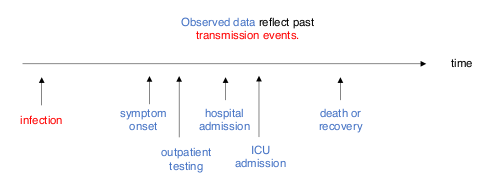
\includegraphics[width=0.90\textwidth]{../lessons/image/22/image08.png}
\caption{\label{fig:22_08} Generation time and serial interval relation.}
\end{figure}

\end{document}
